\chapter{Forest of Moore}

\vspace{\baselineskip}

\begin{paracol}{2}

\begin{enumerate}
    \item Head to the Forest of Moore
\end{enumerate}

\begin{misc}{Path to the Forest of Moore}
    \begin{itemize}
        \item West until you hit a wall
        \item Follow the walls around the northwest out of the trench
        \item Go straight west and count corals on the top edge of the screen
        \item After the third coral, go south
        \item Once you can, go east and north to the emerge point
    \end{itemize}
\end{misc}

\switchcolumn
\begin{steproute}{En Route to the Forest of Moore}
    \insertStep{../Graphics/Steps/142. Guido's Cave 4.jpg}
    \insertStep{../Graphics/Steps/143. Forest of Moore 1.jpg}
\end{steproute}

\switchcolumn
\newpage
\begin{misc}{First Screen Directions}
    \begin{itemize}
        \item Up until the chest and then mostly right
    \end{itemize}
\end{misc}

\begin{enumerate}[resume]
    \item Grab the \pickup{2500 Gil} chest directly north after entering
\end{enumerate}

\switchcolumn
\begin{steproute}{After the 2500 Gil Chest}
    \insertStep{../Graphics/Steps/144. Forest of Moore Enc 1.jpg}
    \insertStep{../Graphics/Steps/145. Forest of More 2.jpg}
    \insertStep{../Graphics/Steps/146. Forest of More 3.jpg}
\end{steproute}

\switchcolumn*
\begin{misc}{Second Screen Directions}
    \begin{itemize}
        \item Right until the first encounter
        \item Up until the second encounter 
        \item Right immediately afterward and grab the chest to the right of the tree
    \end{itemize}
\end{misc}

\switchcolumn
\begin{steproute}{Before the 9500 Gil Chest}
    \insertStep{../Graphics/Steps/147. Forest of Moore Enc 2.jpg}
    \insertStep{../Graphics/Steps/148. Forest of Moore Enc 3.jpg}
\end{steproute}

\switchcolumn
\begin{enumerate}[resume]
    \item Grab the \pickup{9500 Gil} chest on the east side before heading back west to the third screen
\end{enumerate}

\switchcolumn
\begin{steproute}{After the 9500 Gil Chest}
    \insertStep{../Graphics/Steps/149. Forest of Moore Enc 4.jpg}
\end{steproute}

\switchcolumn*
\begin{misc}{Third Screen Directions}
    \begin{itemize}
        \item Mostly up until the encounter
        \item Up until you hit a tree and then keep right until the chest at the top
    \end{itemize}
\end{misc}

\switchcolumn
\begin{steproute}{Before the Morning Star}
    \insertStep{../Graphics/Steps/150. Forest of Moore Enc 5.jpg}
\end{steproute}

\switchcolumn
\begin{enumerate}[resume]
    \item Grab the \pickup{Morning Star} chest at the top of the screen before the fire cutscene
\end{enumerate}

\switchcolumn
\begin{steproute}{Fire Cutscene}
    \insertStep{../Graphics/Steps/151. Forest of Moore 3.jpg}
    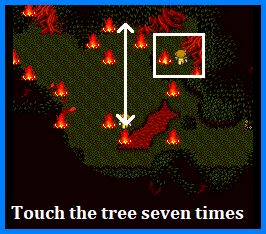
\includegraphics[scale=0.449]{../Graphics/Steps/152. Forest of Moore 4.jpg}
    \insertStep{../Graphics/Steps/153. Forest of Moore 5.jpg}
\end{steproute}

\switchcolumn*
\begin{enumerate}[resume]
    \item After the fire cutscene, heal with the lake
    \item After emerging, grab the \pickup{Flame Shield} chest to the right
    \item Go down and bit and head left (below the tree)
    \item Head up once you see the chest
\end{enumerate}

\switchcolumn
\begin{steproute}{Before Seal Guardians}
    \insertStep{../Graphics/Steps/154. Forest of Moore Enc 6.jpg}
    \insertStep{../Graphics/Steps/155. Forest of Moore Enc 7.jpg}
    \insertStep{../Graphics/Steps/156. Forest of More Enc 8.jpg}
    \insertStep{../Graphics/Steps/157. Forest of Moore Enc 9.jpg}
\end{steproute}

\switchcolumn
\begin{menu}{Before Seal Guardians}
    \varwb
    \begin{jobMenu}
        \lenna Samurai \textbf{(\pointLeft)(\pointDown)} \optimize
        \bartz Chemist \textbf{(\pointUp)(\pointRight)} \ability{!\gilToss} \optimize
        \faris Samurai \textbf{(\pointLeft)(\pointDown)} \equip{\goldShield}
        \galuf Samurai \textbf{(\pointLeft)(\pointDown)} \optimize
    \end{jobMenu}
    \begin{itemMenu}
        \hiPotionMenu \ally{Anyone not near full HP}
    \end{itemMenu}
    \varwe
\end{menu}

\begin{boss}{Seal Guardians}
    \varwb
    \begin{round}{1}
        \bartz \rightCommand{\gilToss}
        \everyoneElse \leftCommand{\gilToss}
    \end{round}
    \varwe
\end{boss}

\begin{boss}{Exdeath}
    \varwb
    \begin{round}{1}
        \galuf Item \then \phoenixDown \space \then \ally{Galuf}
    \end{round}
    \varwe
\end{boss}

\end{paracol}